\documentclass[11pt]{article}
\usepackage[letterpaper]{geometry}
\usepackage{MATH562}

\begin{document}
\noindent \textbf{\Large{Caleb Logemann \\
MATH 562 Numerical Analysis II \\
Homework 1
}}

%\lstinputlisting[language=Matlab]{H01_23.m}
\begin{enumerate}
    \item % #1 Done
        Problem 1.1
        Let $B$ be a $4 \times 4$ matrix to which the following operations are
        applied in the given order.
        \begin{enumerate}
            \item[1.] double column 1
            \item[2.] halve row 3
            \item[3.] add row 3 to row 1
            \item[4.] interchange columns 1 and 4
            \item[5.] subtract row 2 from each other rows
            \item[6.] replace column 4 by column 3
            \item[7.] delete column 1
        \end{enumerate}
        The result can be written as a product of 8 matrices one of which is $B$.
        \begin{enumerate}
            \item[(a)]
                What are the other 7 matrices and what order do they appear in
                the matrix?

                The matrix that doubles column 1 is
                \begin{align*}
                    C &=
                    \begin{bmatrix}
                        2 & 0 & 0 & 0 \\
                        0 & 1 & 0 & 0 \\
                        0 & 0 & 1 & 0 \\
                        0 & 0 & 0 & 1
                    \end{bmatrix}
                    \intertext{when right multiplied.
                        The following matrix halves row 3 when left multiplied.}
                    D &=
                    \begin{bmatrix}
                        1 & 0 & 0 & 0 \\
                        0 & 1 & 0 & 0 \\
                        0 & 0 & .5 & 0 \\
                        0 & 0 & 0 & 1
                    \end{bmatrix}
                    \intertext{The following matrix adds row 3 to the row 1 when left multiplied.}
                    E &= 
                    \begin{bmatrix}
                        1 & 0 & 1 & 0 \\
                        0 & 1 & 0 & 0 \\
                        0 & 0 & 1 & 0 \\
                        0 & 0 & 0 & 1
                    \end{bmatrix}
                    \intertext{The following matrix interchanges columns 1 and 4 when right multiplied.}
                    F &=
                    \begin{bmatrix}
                        0 & 0 & 0 & 1 \\
                        0 & 1 & 0 & 0 \\
                        0 & 0 & 1 & 0 \\
                        1 & 0 & 0 & 0
                    \end{bmatrix}
                    \intertext{The following matrix subtracts row 2 from every other row, when left multiplied.}
                    G &=
                    \begin{bmatrix}
                        1 & -1 & 0 & 0 \\
                        0 & 1 & 0 & 0 \\
                        0 & -1 & 1 & 0 \\
                        0 & -1 & 0 & 1
                    \end{bmatrix}
                    \intertext{The following matrix replaces column 4 with column 3 when right multiplied.}
                    H &=
                    \begin{bmatrix}
                        1 & 0 & 0 & 0 \\
                        0 & 1 & 0 & 0 \\
                        0 & 0 & 1 & 1 \\
                        0 & 0 & 0 & 0
                    \end{bmatrix}
                    \intertext{The following matrix deletes column 1 when right multiplied.}
                    I &=
                    \begin{bmatrix}
                        0 & 0 & 0 \\
                        1 & 0 & 0 \\
                        0 & 1 & 0 \\
                        0 & 0 & 1
                    \end{bmatrix}
                \end{align*}
                The resulting matrix product is given by $GEDBCFHI$, where the
                matrices are given above.

            \item[(b)]
                The result can also be written as a product $ABC$ what are $A$
                and $C$?

                In this case $A$ and $C$ are given by the product of the
                matrices to the left and the right of $B$ in the part (a).
                Therefore
                \begin{align*}
                    A &=
                    \begin{bmatrix}
                        1 & -1 & 0.5 & 0 \\
                        0 &  1 & 0 & 0 \\
                        0 & -1 & 0.5 & 0 \\
                        0 & -1 & 0 & 1
                    \end{bmatrix} \\
                    C &=
                    \begin{bmatrix}
                        0 & 0 & 0 \\
                        1 & 0 & 0 \\
                        0 & 1 & 1 \\
                        0 & 0 & 0
                    \end{bmatrix}
                \end{align*}

        \end{enumerate}

    \item % #2 done
        Show that if a matrix $A \in \CC^{m \times m}$ is upper triangular and
        unitary, then it is diagonal.

        \begin{proof}
            Let $A \in \CC^{m \times m}$ be unitary and upper triangular.
            I will denote $A$ be its entries $a_{ij}$ and by its columns as
            vectors $\v{a_j}$.
            The fact that $A$ is upper triangular implies that $a_{ij} = 0$,
            for $i > j$.
            Since $A$ is unitary, $AA^* = I$ or $\v{a}_j^*\v{a}_i = 0$ for
            $i \neq j$ and $\v{a}_j^*\v{a}_i = 1$ for $i = j$.
            We will procede by induction. 
            Consider $\v{a}_1^*\v{a}_j = 0$ for $j = 2, \ldots, m$.
            However since $A$ is upper triangular $\v{a}_1 = \v{e}_1$, thus
            $\v{a}_1^*\v{a}_j = a_{1j}$.
            Therefore $a_{1j} = 0$ for $j = 2, \ldots, m$.
            Now assume that $a_{ij} = 0$ for $i = 1, \ldots, k - 1$ and
            $j = i + 1, \ldots, m$.
            Consider $\v{a}_k^* \v{a}_j = 0$ for $j = k+1, \ldots, m$.
            However we know that $a_{ik} = 0$ for $i < k$ and $a_{ik} = 0$ for
            $i > k$, therefore $\v{a}_k = \v{e}_k$.
            This implies that $\v{a}_k^* \v{a}_j = a_{kj}$.
            We can now conclude that $a_{kj} = 0$ for $j = k+1, \ldots, m$.
            Now mathematical induction implies that $a_{ij} = 0$ for
            $i = 1, \ldots, m$ and $j = i+1, \ldots, m$.
            This means that all entries above the diagonal are zero, and thus
            $A$ is a diagonal matrix.
            Essential each row can be shown to be zero except on the diagonal
            by noting that the previous row is zero everywhere except the
            diagonal.
        \end{proof}

    \item % #3 Problem 2.3 page 15 Done
        Let $A \in \CC^{m \times m}$ be Hermitian, that is $A = A^*$.
        Suppose that $A\v{x} = \lambda\v{x}$, where $\v{x} \in \CC^{m \times m}$
        and $\lambda \in \CC$, so $\v{x}$ is an eigenvector and $\lambda$ is an
        eigenvalue.
        \begin{enumerate}
            \item[(a)]
                Prove that $\lambda$ must be real.

                \begin{proof}
                    Consider $\v{x}^* A \v{x}$.
                    \begin{align*}
                        \p{\v{x}^* A} \v{x} &= \v{x}^* \p{A \v{x}} \\
                        \p{A^* \v{x}}^* \v{x} &= \v{x}^* \p{A \v{x}} \\
                        \p{\lambda \v{x}}^* \v{x} &= \v{x}^* \p{\lambda \v{x}} \\
                        \overline{\lambda} \v{x}^* \v{x} &= \lambda \v{x}^*\v{x}  \\
                        \overline{\lambda} &= \lambda
                    \end{align*}
                    Since $\overline{\lambda} = \lambda$, $\lambda$ must be real. 
                \end{proof}

            \item[(b)]
                Prove that if $\v{x}$ and $\v{y}$ are eigenvectors
                corresponding to different eigenvalues, then $\v{x}$ and
                $\v{y}$ are orthogonal.

                \begin{proof}
                    Let $\lambda_x$ and $\lambda_y$ be the eigenvalues corresponding
                    to $\v{x}$ and $\v{y}$ respectively, that is
                    $A\v{x} = \lambda_x\v{x}$, $A\v{y} = \lambda_y\v{y}$, and
                    $\lambda_x \neq \lambda_y$.
                    Since $A$ is Hermitian, we have just shown that
                    $\lambda_x, \lambda_y \in \RR$.
                    Also because $A$ is Hermitian
                    \begin{align*}
                        A &= A^* \\
                        \v{x}^* A &= \v{x}^* A^* \\
                        \v{x}^* A &= \p{A\v{x}}^*.
                        \intertext{Since $\v{x}$ is an eigenvector}
                        \v{x}^* A &= \p{\lambda_x \v{x}}^*
                        \intertext{Since $\lambda_x \in \RR$}
                        \v{x}^* A &= \lambda_x \v{x}^* \\
                        \v{x}^* A \v{y} &= \lambda_x \v{x}^* \v{y} \\
                        \v{x}^* \lambda_y \v{y} &= \lambda_x \v{x}^* \v{y} \\
                        \p{\lambda_y - \lambda_x} \v{x}^* \v{y} &= 0
                        \intertext{Since $\lambda_x \neq \lambda_y$, $\lambda_y - \lambda_x \neq 0$.}
                        \v{x}^* \v{y} &= 0
                    \end{align*}
                    Therefore $\v{x}$ and $\v{y}$ are orthogonal.
                \end{proof}
        \end{enumerate}

    \item % #4 Problem 2.6 page 16 Done
        If $\v{u}, \v{v} \in \RR^m$, then $A = I + \v{u}\v{v}^T$ is called a
        rank one perturbation of the identity.
        \begin{enumerate}
            \item[(a)]
                Show that if $A$ is invertible, then it's inverse has the form
                $A^{-1} = I + \alpha \v{u}\v{v}^T$, and give an expression for
                the scalar $\alpha$.

                First let us find an expression for $\alpha$.
                \begin{align*}
                    I &= AA^{-1} \\
                      &= \p{I + \v{u}\v{v}^T}\p{I + \alpha \v{u}\v{v}^T} \\
                      &= I + \alpha \v{u}\v{v}^T + \v{u}\v{v}^T + \alpha \v{u}\v{v}^T \v{u}\v{v}^T \\
                      &= I + \p{\alpha + 1 + \alpha \v{v}^T\v{u}}\v{u}\v{v}^T
                    \intertext{In order for this equality to be true}
                    0 &= \alpha + 1 + \alpha \v{v}^T\v{u} \\
                    \alpha &= -\frac{1}{1 + \v{v}^T\v{u}}
                \end{align*}
                \begin{proof}
                    If $A$ is invertible then $A^{-1}$ exists and is unique.
                    Consider the matrix $B = I + \alpha \v{u}\v{v}^T$, where
                    $\alpha = -\frac{1}{1 + \v{v}^T\v{u}}$, then the following
                    can be stated.
                    \begin{align*}
                        AB &= \p{I + \v{u}\v{v}^T}\p{I + \alpha \v{u}\v{v}^T} \\
                        &= I + \alpha \v{u}\v{v}^T + \v{u}\v{v}^T + \alpha \v{u}\v{v}^T \v{u}\v{v}^T \\
                        &= I + \p{\alpha + 1 + \alpha \v{v}^T\v{u}}\v{u}\v{v}^T \\
                        &= I + \p{\p{1 + \v{v}^T\v{u}}\p{-\frac{1}{1 + \v{v}^T\v{u}}} + 1}\v{u}\v{v}^T \\
                        &= I + \p{-1 + 1}\v{u}\v{v}^T \\
                        &= I \\
                    \end{align*}
                    Similarly it can be shown that $BA = I$.
                    Thus $B$ is an inverse of $A$, and since the inverse is
                    unique $B = I + \alpha \v{u}\v{v}^T$ is the inverse of $A$.
                    Therefore if $A$ is invertible it's inverse will be of the
                    form $I + \alpha \v{u}\v{v}^T$.
                \end{proof}

            \item[(b)]
                If $A$ is not invertible than $\v{v}^T \v{u} = -1$, otherwise
                $I + \alpha \v{u}\v{v}^T$, where
                $\alpha = -\frac{1}{1 + \v{v}^T\v{u}}$ would be an inverse.
                In this case $\nullspace(A) = \spanspace\set{\v{u}}$.
                Note that
                \begin{align*}
                    A(c\v{u}) &= \p{I + \v{u}\v{v}^T}(c\v{u}) \\
                            &= c\v{u} + c\v{u}\v{v}^T\v{u} \\
                            &= c\v{u} - c\v{u} \\
                            &= \v{0}
                \end{align*}
                for any $c \in \RR$.
                Thus any multiple of $\v{u}$ is in $\nullspace(A)$.
        \end{enumerate}

    \item % #5 Problem 3.2 page 24 Done
        Let $\norm{\cdot}$ denote any norm on $\CC^m$ and also the corresponding
        induced norm on $\CC^{m \times m}$, so that
        $\norm{A\v{x}} \le \norm{A}\norm{\v{x}}$.
        Show that $\rho(A) \le \norm{A}$, where
        $\rho(A) = \max{\abs{\lambda}:\text{where $\lambda$ is an eigenvalue of $A$}}$
        is the spectral radius of $A$.

        \begin{proof}
            Let $\v{x}$ be an eigenvector of $A$ with corresponding eigenvalue
            $\lambda$, such that $\abs{\lambda} = \rho(A)$, that is $\v{x}$ is
            the eigenvector corresponding to the eigenvalue whose magnitude is
            the spectral radius.
            Consider $\norm{A\v{x}}$
            \begin{align*}
                \norm{A\v{x}} &= \norm{\lambda \v{x}} \\
                &= \abs{\lambda} \norm{\v{x}} \\
                &= \rho(A) \norm{\v{x}}
            \end{align*}
            Also note that $\norm{A\v{x}} \le \norm{A}\norm{\v{x}}$, therefore
            \begin{align*}
                \rho(A) \norm{\v{x}} &\le \norm{A}\norm{\v{x}} \\
                \rho(A) &\le \norm{A}
            \end{align*}
            Since $\norm{\v{x}} \neq 0$, because $\v{x}$ is an eigenvector.
        \end{proof}

    \item % #6 Done
        Let $\theta \in \p{0, 2\pi}$ and define the matrix
        $Q \in \RR^{2 \times 2}$ by
        \begin{align*}
            Q =
            \begin{bmatrix}
                \cos{\theta} & -\sin{\theta} \\
                \sin{\theta} & \cos{\theta}
            \end{bmatrix}.
        \end{align*}
        Show that $\v{y} = Q\v{x}$ is the vector obtained by rotating vector
        $\v{x}$ by $\theta$ radians.
        % Hint use polar coordinates for the components of your vector

        \begin{proof}
            Let $\v{x} \in \RR^2$, have entries $x_1$ and $x_2$, then the
            following statements are true $x_1 = r\cos{\phi}$ and
            $x_2 = r\sin{\phi}$, where $r = \sqrt{x_1^2 + x_2^2}$ is the radius
            or length of the vector and $\phi = \arctan{\frac{x_1}{x_2}}$ is the
            angle between the vector and the x-axis.
            If the vector is in the third or fourth quadrants the angle must be shifted
            as necessary.
            Now the vector $\v{y}$ can be computed as follows.
            \begin{align*}
                \v{y} &= Q\v{x} \\
                &= 
                \begin{bmatrix}
                    \cos{\theta} & -\sin{\theta} \\
                    \sin{\theta} & \cos{\theta}
                \end{bmatrix}
                \begin{bmatrix}
                    r\cos{\phi}  \\
                    r\sin{\phi} 
                \end{bmatrix} \\
                &= 
                \begin{bmatrix}
                    r\p{\cos{\theta}\cos{\phi} - \sin{\theta}\sin{\phi}} \\
                    r\p{\sin{\theta}\cos{\phi} + \cos{\theta}\sin{\phi}}
                \end{bmatrix}
                \intertext{Using some trigonomtric identities}
                \v{y} &= 
                \begin{bmatrix}
                    r\cos{\theta + \phi} \\
                    r\sin{\theta + \phi}
                \end{bmatrix}
            \end{align*}
            However this is just vector $\v{x}$ except rotated by $\theta$ radians.
            It has the same length or radius, but the angle was changed by $\theta$.
        \end{proof}

    \item % #7 Done
        Below I have shown my function for finding the SVD decomposition of
        a $2 \times 2$ real matrix. The code does use the circle\_image and arrow
        functions provided in class.

        \lstinputlisting[language=Matlab]{H01.m}
        \lstinputlisting[language=Matlab]{SVD2D.m}

        This code produces the following two figures
        for
        \begin{align*}
            A =
            \begin{bmatrix}
                1 & 2 \\
                0 & 2
            \end{bmatrix}
        \end{align*}
        and
        \begin{align*}
            A =
            \begin{bmatrix}
                1 & 1 \\
                2 & 2
            \end{bmatrix}
        \end{align*}
        respectively.
        \begin{center}
            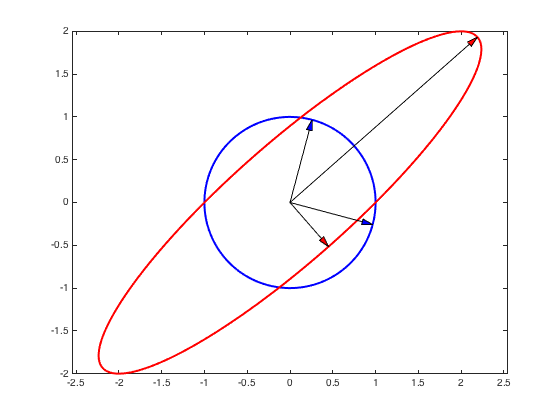
\includegraphics[scale=.5]{Figures/01_7_1.png} \\
            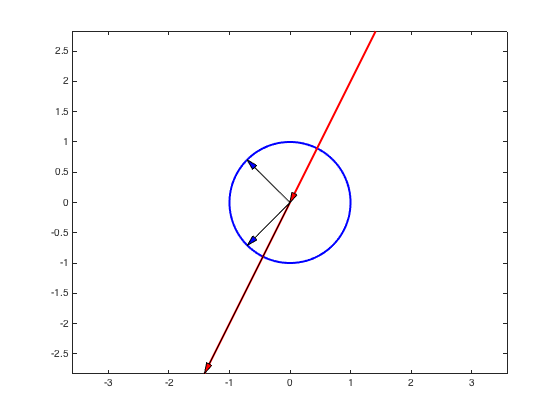
\includegraphics[scale=.5]{Figures/01_7_2.png}
        \end{center}

\end{enumerate}
\end{document}
